\documentclass[12pt,a4paper]{article}
\usepackage[utf8]{vietnam}
\usepackage{amsmath,amssymb}
\usepackage{geometry}
\geometry{top=1.5cm,bottom=1.2cm,left=1.4cm,right=1.4cm,headheight=28pt,headsep=12pt,footskip=18pt}
\usepackage{tikz}
\usepackage{xcolor}
\usepackage{enumerate}
\usepackage{graphicx}
\usepackage[version=4]{mhchem}
\usepackage{fancyhdr}
\usepackage{ex_test}

\renewcommand{\baselinestretch}{1.0}
\setlength{\parskip}{1pt}

\definecolor{hfRed}{RGB}{211,47,47}
\definecolor{hfGreen}{RGB}{139,195,144}

\pagestyle{fancy}
\fancyhf{}
\fancyhead[L]{\small\itshape\color{hfRed} Tài liệu lưu hành nội bộ}
\fancyhead[R]{\small\itshape\color{hfRed} Thầy \textbf{TRẦN VĂN THẠNH} - 0777.470.803}
\renewcommand{\headrulewidth}{0.8pt}
\renewcommand{\headrule}{\hbox to\headwidth{\color{hfGreen}\leaders\hrule height \headrulewidth\hfill}}

\fancyfoot[L]{\small\itshape\color{hfRed} CS1: 6/15 Nguyễn Hoàng, P. Kim Long, TP Huế \quad|\quad CS2: 24 Đặng Thái Thân, TP Huế}
\fancyfoot[R]{\small\bfseries\color{hfRed} Trang \thepage}
\renewcommand{\footrulewidth}{0.8pt}
\renewcommand{\footrule}{\hbox to\headwidth{\color{hfGreen}\leaders\hrule height \footrulewidth\hfill}}

\fancypagestyle{firstpage}{
  \fancyhf{}
  \renewcommand{\headrulewidth}{0pt}
  \fancyfoot[L]{\small\itshape\color{hfRed} CS1: 6/15 Nguyễn Hoàng, P. Kim Long, TP Huế \quad|\quad CS2: 24 Đặng Thái Thân, TP Huế}
  \fancyfoot[R]{\small\bfseries\color{hfRed} Trang \thepage}
  \renewcommand{\footrulewidth}{0.8pt}
  \renewcommand{\footrule}{\hbox to\headwidth{\color{hfGreen}\leaders\hrule height \footrulewidth\hfill}}
}

\begin{document}
\thispagestyle{firstpage}

\noindent
\begin{minipage}[t]{0.45\textwidth}
	\centering\fontsize{10pt}{12pt}\selectfont
	\textbf{SỞ GD\&ĐT THÀNH PHỐ HUẾ}\\
	\textbf{TRƯỜNG THPT PHONG ĐIỀN}\\
	\textbf{ĐỀ CHÍNH THỨC}\\
	\textit{(Đề thi có 04 trang)}
\end{minipage}\hfill
\begin{minipage}[t]{0.53\textwidth}
	\centering\small
	\textbf{KIỂM TRA GIỮA HỌC KỲ I -- NĂM HỌC 2025 - 2026}\\
	\textbf{MÔN: HOÁ HỌC 11 CTST}\\
	\textit{Thời gian làm bài: 45 phút (không kể thời gian phát đề)}\\
	\fbox{\textbf{MÃ ĐỀ: 504}}
\end{minipage}

\smallskip
\begin{center}
	{\color{hfRed}\textbf{\large (BẢN GIÁO VIÊN -- CÓ LỜI GIẢI CHI TIẾT)}}
\end{center}

\smallskip
\noindent\hrulefill
\smallskip

\noindent\textbf{Họ, tên thí sinh:} \dotfill\ \textbf{Lớp:} \dotfill\ \textbf{Số báo danh:} \dotfill

\smallskip
\noindent\textit{(Cho biết nguyên tử khối: H = 1; C = 12; N = 14; O = 16; Na = 23; S = 32; Cl = 35,5; Fe = 56).}
\smallskip

\noindent
\textbf{PHẦN I. Câu trắc nghiệm nhiều phương án lựa chọn.}\\
\textit{Thí sinh trả lời từ câu 1 đến câu 12. Mỗi câu hỏi thí sinh chỉ chọn một phương án.}

\Opensolutionfile{ans}[ans-hoa11-ma504gv]

\begin{ex}
Cân bằng hóa học là một cân bằng
\choice
{Đứng yên}
{Tĩnh}
{Cố định}
{\True Động}
\loigiai{
Cân bằng hóa học là cân bằng động vì ở trạng thái cân bằng, phản ứng thuận và phản ứng nghịch vẫn tiếp tục xảy ra với tốc độ bằng nhau ($v_t = v_n \neq 0$).\\
\textbf{Chọn D.}}
\end{ex}

\begin{ex}
Trong thí nghiệm đốt cháy sulfur (S) trong không khí, hiện tượng nào sau đây có thể được quan sát?
\choice
{Sulfur cháy với ngọn lửa màu đỏ và sinh ra khói trắng}
{\True Sulfur cháy với ngọn lửa màu xanh và sinh ra khí không màu, mùi hắc}
{Sulfur cháy với ngọn lửa màu tím và sinh ra khí không mùi}
{Sulfur cháy với ngọn lửa màu vàng nhạt và sinh ra khí có mùi ngọt}
\loigiai{
Sulfur cháy trong không khí với ngọn lửa nhỏ màu xanh nhạt, sinh ra sulfur dioxide ($\ce{SO2}$) là chất khí không màu, có mùi hắc: $\ce{S + O2 ->[t^\circ] SO2}$.\\
\textbf{Chọn B.}}
\end{ex}

\begin{ex}
Nạp đầy khí amoniac vào bình thuỷ tinh trong suốt, đậy bình $\ce{NH3}$ bằng nút cao su có ống thuỷ tinh vuốt nhọn xuyên qua. Nhúng đầu ống thuỷ tinh vào một chậu thuỷ tinh chứa nước có pha thêm dung dịch phenolphthalein. Một lát sau, nước trong chậu phun vào bình thành những tia có màu hồng. Thí nghiệm này chứng tỏ được:
\choice
{$\ce{NH3}$ là chất khí.}
{$\ce{NH3}$ tan nhiều trong nước.}
{$\ce{NH3}$ có mùi khai.}
{\True $\ce{NH3}$ có tính bazơ và tan nhiều trong nước.}
\loigiai{
- Khí $\ce{NH3}$ tan rất nhiều trong nước làm áp suất trong bình giảm mạnh, kéo nước từ chậu phun mạnh vào bình thành các tia.\\
- Nước phun vào có màu hồng chứng tỏ dung dịch $\ce{NH3}$ có tính base (làm phenolphthalein chuyển màu hồng).\\
Do đó, thí nghiệm chứng minh $\ce{NH3}$ có tính base và tan nhiều trong nước.\\
\textbf{Chọn D.}}
\end{ex}

\begin{ex}
Nitrogen monoxide được tạo thành khi mưa dông kèm theo sấm sét do phản ứng giữa nitrogen và oxygen trong không khí được gọi là
\choice
{$\ce{NO_x}$ nhiên liệu.}
{$\ce{NO_x}$ tức thời.}
{\True $\ce{NO_x}$ tự nhiên.}
{$\ce{NO_x}$ nhiệt.}
\loigiai{
Khí $\ce{NO}$ được sinh ra do hiện tượng sấm sét tự nhiên giữa nitrogen và oxygen trong khí quyển được gọi là $\ce{NO_x}$ tự nhiên.\\
\textbf{Chọn C.}}
\end{ex}

\begin{ex}
Cho các nhận định sau về cấu tạo phân tử nitric acid:\\
(a) Liên kết $\ce{O - H}$ phân cực về oxygen.\\
(b) Nguyên tử N có số oxi hóa là $+5$.\\
(c) Nguyên tử N có hóa trị bằng IV.\\
(d) Liên kết cho -- nhận $\ce{N -> O}$ kém bền.\\
Số nhận định đúng là
\choice
{\True 4.}
{1.}
{2.}
{3.}
\loigiai{
- (a) Đúng vì độ âm điện O ($3{,}44$) lớn hơn H ($2{,}20$) nên liên kết $\ce{O - H}$ phân cực về phía O.\\
- (b) Đúng vì trong $\ce{HNO3}$, N có số oxi hóa $+5$.\\
- (c) Đúng vì N ở chu kì 2 có 4 orbital hóa trị nên hóa trị tối đa bằng IV.\\
- (d) Đúng vì liên kết cho -- nhận $\ce{N -> O}$ kém bền nên $\ce{HNO3}$ dễ bị phân hủy giải phóng $\ce{NO2}$ và $\ce{O2}$.\\
Cả 4 nhận định đều đúng.\\
\textbf{Chọn A.}}
\end{ex}

\begin{ex}
Đâu là phát biểu của thuyết Bronsted-Lowry?
\choice
{Acid là chất nhận proton, base là chất cho proton}
{Cả acid và base đều là chất nhận proton}
{\True Acid là chất cho proton, base là chất nhận proton}
{Cả acid và base đều là chất cho proton}
\loigiai{
Theo thuyết Brønsted -- Lowry: Acid là chất cho proton ($\ce{H+}$), base là chất nhận proton ($\ce{H+}$).\\
\textbf{Chọn C.}}
\end{ex}

\begin{ex}
Xét cân bằng: $\ce{N2(g) + 3H2(g) <=> 2NH3(g)}$. Biểu thức hằng số cân bằng của phản ứng là:
\choice
{$K = \frac{[\ce{N2}][\ce{H2}]}{[\ce{NH3}]}$}
{$K = \frac{[\ce{NH3}]}{[\ce{N2}][\ce{H2}]}$}
{\True $K = \frac{[\ce{NH3}]^2}{[\ce{N2}][\ce{H2}]^3}$}
{$K = \frac{[\ce{N2}][\ce{H2}]^3}{[\ce{NH3}]^2}$}
\loigiai{
Biểu thức hằng số cân bằng $K_C$:
\[ K = \frac{[\ce{NH3}]^2}{[\ce{N2}][\ce{H2}]^3} \]
\textbf{Chọn C.}}
\end{ex}

\begin{ex}
Hợp chất nào sau đây của sulfur được sử dụng để khử trùng và tẩy trắng trong công nghiệp?
\choice
{\True $\ce{SO2}$}
{$\ce{H2SO4}$}
{$\ce{S8}$}
{$\ce{H2S}$}
\loigiai{
$\ce{SO2}$ (sulfur dioxide) được dùng để khử trùng, diệt nấm mốc và tẩy trắng bột giấy, sợi vải trong công nghiệp.\\
\textbf{Chọn A.}}
\end{ex}

\begin{ex}
Trong tự nhiên luôn diễn ra các quá trình chuyển hóa nitrogen từ dạng này sang dạng khác theo...
\choice
{Một chu trình tuần hoàn không khép kín}
{\True Một chu trình tuần hoàn khép kín}
{Một chu trình ngẫu nhiên}
{Một chu trình không tuần hoàn}
\loigiai{
Trong tự nhiên, nitrogen liên tục luân chuyển qua lại giữa khí quyển, đất, sinh vật và nước theo một chu trình tuần hoàn khép kín (chu trình nitrogen).\\
\textbf{Chọn B.}}
\end{ex}

\begin{ex}
pH là
\choice
{Chỉ số đánh giá độ acid của một dung dịch}
{\True Chỉ số đánh giá độ acid hay độ base của một dung dịch}
{Chỉ số đánh giá độ base của một dung dịch}
{Chỉ số đánh giá các chất điện li mạnh}
\loigiai{
pH là chỉ số được dùng để đánh giá độ acid hay độ base của một dung dịch ($\text{pH} = -\log[\ce{H+}] $).\\
\textbf{Chọn B.}}
\end{ex}

\begin{ex}
Tính chất nào sau đây là tính chất vật lý của sulfur (S)?
\choice
{Là chất khí không màu}
{\True Là chất rắn màu vàng, không tan trong nước}
{Tan tốt trong nước}
{Dễ bay hơi ở nhiệt độ thường}
\loigiai{
Ở điều kiện thường, sulfur là chất rắn màu vàng, giòn, không tan trong nước.\\
\textbf{Chọn B.}}
\end{ex}

\begin{ex}
Cho các nhận định sau về tính chất hoá học của nitric acid: (1) có tính acid mạnh; (2) có tính acid yếu; (3) có tính oxi hoá mạnh; (4) có tính khử mạnh. Số nhận định đúng là
\choice
{4.}
{1.}
{\True 2.}
{3.}
\loigiai{
Nitric acid ($\ce{HNO3}$) có tính acid mạnh và có tính oxi hóa mạnh (do N có số oxi hóa cao nhất $+5$). Do đó có 2 nhận định đúng: (1) và (3).\\
\textbf{Chọn C.}}
\end{ex}

\Closesolutionfile{ans}

\bigskip
\noindent
\textbf{PHẦN II. Câu trắc nghiệm đúng sai. (2 điểm)}\\
\textit{Trong mỗi ý a), b), c), d) ở mỗi câu, thí sinh chọn đúng hoặc sai. Điểm tối đa của 01 câu hỏi là 1 điểm:}\\
\textit{- Thí sinh chỉ lựa chọn chính xác 01 ý trong 1 câu hỏi được 0,1 điểm.}\\
\textit{- Thí sinh chỉ lựa chọn chính xác 02 ý trong 1 câu hỏi được 0,25 điểm.}\\
\textit{- Thí sinh chỉ lựa chọn chính xác 03 ý trong 1 câu hỏi được 0,5 điểm.}\\
\textit{- Thí sinh chỉ lựa chọn chính xác 04 ý trong 1 câu hỏi được 1 điểm.}

\begin{ex}
Ammonium nitrate được dùng làm phân đạm. Năm 2020, một vụ nổ tại thủ đô Beirut, Lebanon đã cướp đi sinh mạng của hàng trăm người. Nguyên nhân của vụ nổ được do sự phân huỷ 2750 tấn ammonium nitrate trên một tàu hàng bỏ hoang theo phương trình hoá học sau:
\[ \ce{NH4NO3(s) -> N2O(g) + 2H2O(g)} \quad \Delta_r H_{298}^\circ = -36\text{ kJ} \]
\choiceTF
{a) Phản ứng (1) là phản ứng thu nhiệt.}
{b) Dung dịch muối Ammonium nitrate phản ứng với dung dịch base đặc, nóng thoát ra chất khí làm quỳ tím ẩm hoá đỏ.}
{\True c) Khi bón phân đạm ammonium nitrate nhiều sẽ gây hiện tượng chua đất.}
{\True d) Nhiệt của vụ nổ trên tương đương với nhiệt toả ra 1062 tấn thuốc nổ TNT. (biết 1 kg thuốc nổ TNT phát nổ toả ra $1{,}165 \cdot 10^6\text{ J}$).}
\loigiai{
a) Sai vì $\Delta_r H_{298}^\circ = -36\text{ kJ} < 0$, phản ứng tỏa nhiệt.\\
b) Sai vì phản ứng $\ce{NH4+ + OH- ->[t^\circ] NH3 ^ + H2O}$ sinh ra khí $\ce{NH3}$ làm quỳ tím ẩm hóa xanh.\\
c) Đúng vì ion $\ce{NH4+}$ thủy phân tạo $\ce{H3O+}$: $\ce{NH4+ + H2O <=> NH3 + H3O+}$, làm giảm pH của đất gây chua đất.\\
d) Đúng. Số mol $\ce{NH4NO3} = \frac{2750 \times 10^6\text{ g}}{80\text{ g/mol}} = 34\,375\,000\text{ mol}$.\\
Nhiệt tỏa ra: $Q = 34\,375\,000 \times 36 \times 10^3\text{ J} = 1{,}2375 \cdot 10^{12}\text{ J}$.\\
Khối lượng TNT tương đương:
\[ m_{\text{TNT}} = \frac{1{,}2375 \cdot 10^{12}}{1{,}165 \cdot 10^6} \approx 1\,062\,232\text{ kg} \approx 1062\text{ tấn}. \]}
\end{ex}

\begin{ex}
Một học sinh làm thí nghiệm xác định pH của đất như sau: lấy một lượng đất cho vào nước rồi lọc lấy phần dung dịch. Dùng máy đo pH đo được $\text{pH} = 4{,}69$.
\choiceTF
{\True a) Môi trường của dung dịch là acid.}
{\True b) Loại đất trên được gọi là đất chua. Để giảm độ chua cho đất có thể bón vôi.}
{c) Dung dịch trong cốc có $[\ce{OH-}] > [\ce{H+}]$ vì $\text{pOH} > \text{pH}$.}
{d) Nồng độ $[\ce{H+}]$ trong cốc lớn hơn 0,001.}
\loigiai{
a) Đúng vì $\text{pH} = 4{,}69 < 7 \implies$ môi trường acid.\\
b) Đúng vì đất có $\text{pH} < 7$ là đất chua, bón vôi ($\ce{CaO}, \ce{Ca(OH)2}$) để trung hòa lượng acid dư, giảm chua cho đất.\\
c) Sai vì $\text{pH} = 4{,}69 \implies \text{pOH} = 9{,}31 > \text{pH} \implies [\ce{H+}] \approx 2{,}04 \cdot 10^{-5}\text{ M} > [\ce{OH-}] \approx 4{,}9 \cdot 10^{-10}\text{ M}$.\\
d) Sai vì $[\ce{H+}] = 10^{-4{,}69} \approx 2{,}04 \cdot 10^{-5}\text{ M} < 0{,}001\text{ M}$ ($10^{-3}\text{ M}$).}
\end{ex}

\bigskip
\noindent
\textbf{PHẦN III: Câu trắc nghiệm yêu cầu trả lời ngắn. (2 điểm)}\\
\textit{Thí sinh trả lời từ câu 1 đến câu 4.}

\begin{ex}
Tổng số liên kết $\sigma$ và số liên kết $\pi$ trong phân tử nitrogen là bao nhiêu?
\shortans{3}
\loigiai{
Phân tử nitrogen ($\ce{N2}$) có công thức cấu tạo $\ce{N#N}$ gồm 1 liên kết $\sigma$ và 2 liên kết $\pi$.\\
Tổng số liên kết $\sigma$ và $\pi = 1 + 2 = 3$.\\
\textbf{Đáp án: 3.}}
\end{ex}

\begin{ex}
Để giảm thải lượng khí thải $\ce{SO2}$ ra môi trường, trong các biện pháp sau:\\
(1) Sử dụng nguồn nhiên liệu sinh học thân thiện với môi trường như hydrogen, ethanol.\\
(2) Sử dụng nguồn năng lượng hóa thạch.\\
(3) Sử dụng nguồn năng lượng tái tạo như năng lượng mặt trời, năng lượng gió, mưa, sóng biển, thủy triều, địa nhiệt.\\
(4) Xử lý khí thải công nghiệp trước khi thải ra môi trường.\\
Cần thực hiện biện pháp nào trong số các biện pháp trên?
\shortans{3}
\loigiai{
- (1) Nhiên liệu sinh học không chứa lưu huỳnh $\implies$ giảm thải $\ce{SO2}$ (thực hiện).\\
- (2) Năng lượng hóa thạch phát thải nhiều $\ce{SO2}$ (không thực hiện).\\
- (3) Năng lượng tái tạo sạch không phát thải $\ce{SO2}$ (thực hiện).\\
- (4) Xử lý khí thải công nghiệp giúp loại bỏ $\ce{SO2}$ trước khi xả thải (thực hiện).\\
Có 3 biện pháp cần thực hiện: (1), (3), (4).\\
\textbf{Đáp án: 3.}}
\end{ex}

\begin{ex}
Dịch vị dạ dày của con người có chứa hydrochloric acid ($\ce{HCl}$), với pH dao động trong khoảng 2-4. Những người bị mắc bệnh viêm loét dạ dày, tá tràng thường có $\text{pH} < 2$. Nabica (có thành phần chính là $\ce{NaHCO3}$) là một loại thuốc được dùng để trung hoà bớt lượng acid trong dạ dày của những bệnh nhân có pH trong dạ dày thấp và thường được uống trước bữa ăn. Giả sử một bệnh nhân bị đau dạ dày đã uống $0{,}504\text{ gam}$ bột $\ce{NaHCO3}$. Hãy tính số mol $\ce{HCl}$ đã được trung hòa.
\shortans{0{,}006}
\loigiai{
Số mol $\ce{NaHCO3} = \frac{0{,}504}{84} = 0{,}006\text{ mol}$.\\
Phương trình phản ứng: $\ce{NaHCO3 + HCl -> NaCl + CO2 ^ + H2O}$.\\
Theo phương trình: $n_{\ce{HCl}} = n_{\ce{NaHCO3}} = 0{,}006\text{ mol}$.\\
\textbf{Đáp án: 0,006.}}
\end{ex}

\begin{ex}
Cho các phát biểu sau:\\
(a) Trong không khí, Nitrogen chiếm khoảng 78\% về thể tích.\\
(b) Trong bầu khí quyển, khi có sấm chớp, khí nitrogen tạo các nitrogen oxide, là một nguyên nhân làm cho nước mưa có tính acid.\\
(c) Trong phản ứng giữa $\ce{N2}$ và $\ce{H2}$ thì $\ce{N2}$ là chất khử.\\
(d) Phần lớn Nitrogen được sử dụng để tổng hợp $\ce{NH3}$, từ đó sản xuất nitric acid, phân bón.\\
Số phát biểu đúng là bao nhiêu?
\shortans{3}
\loigiai{
- (a) Đúng vì $\ce{N2}$ chiếm khoảng 78\% thể tích không khí.\\
- (b) Đúng vì sấm sét sinh ra $\ce{NO} \to \ce{NO2} \to \ce{HNO3}$ gây mưa acid.\\
- (c) Sai vì $\ce{N2 + 3H2 <=> 2NH3}$, số oxi hóa của N giảm từ 0 xuống $-3$ nên $\ce{N2}$ là chất oxi hóa.\\
- (d) Đúng vì phần lớn $\ce{N2}$ dùng tổng hợp $\ce{NH3}$ sản xuất phân bón và $\ce{HNO3}$.\\
Có 3 phát biểu đúng: (a), (b), (d).\\
\textbf{Đáp án: 3.}}
\end{ex}

\bigskip
\noindent
\textbf{PHẦN IV: Tự luận (3 điểm)}

\begin{ex}
\textbf{(0,5 điểm)} Giải thích vì sao khi mở nắp chai nước có gas, dung dịch bị sủi bọt mạnh, sau đó giảm dần.
\loigiai{
- Trong chai nước có gas đóng kín, khí $\ce{CO2}$ được nén ở áp suất cao hòa tan trong nước ngọt theo cân bằng: $\ce{CO2(aq) <=> CO2(g)}$.\\
- Khi mở nắp chai, áp suất khí trên bề mặt dung dịch giảm đột ngột về áp suất khí quyển. Theo định luật Henry, độ tan của khí $\ce{CO2}$ giảm mạnh khi áp suất giảm, làm cho một lượng lớn khí $\ce{CO2}$ thoát ra khỏi dung dịch gây sủi bọt mạnh.\\
- Sau một thời gian, lượng $\ce{CO2}$ thoát ra đã gần hết và hệ đạt tới trạng thái cân bằng mới ở áp suất khí quyển nên hiện tượng sủi bọt giảm dần rồi dừng lại.}
\end{ex}

\begin{ex}
\textbf{(0,5 điểm)} Một nhà máy thải ra $1000\text{ m}^3$ khí chứa $0{,}05\%$ thể tích $\ce{SO2}$ mỗi ngày. Tính khối lượng $\ce{SO2}$ (tính bằng kg) thải ra trong ngày (ở đktc).
\loigiai{
- Thể tích khí $\ce{SO2}$ thải ra mỗi ngày: $V_{\ce{SO2}} = 1000\text{ m}^3 \times 0{,}05\% = 0{,}5\text{ m}^3 = 500\text{ Lít}$.\\
- Số mol $\ce{SO2}$ thải ra ở đktc ($22{,}4\text{ L/mol}$): $n_{\ce{SO2}} = \frac{500}{22{,}4} \approx 22{,}3214\text{ mol}$.\\
- Khối lượng $\ce{SO2}$ thải ra mỗi ngày:
\[ m_{\ce{SO2}} = 22{,}3214\text{ mol} \times 64\text{ g/mol} \approx 1428{,}57\text{ gam} \approx 1{,}429\text{ kg}. \]
\textit{(Ghi chú: Nếu tính theo đkc $24{,}79\text{ L/mol}$ thì $m_{\ce{SO2}} = \frac{500}{24{,}79} \times 64 \approx 1290{,}84\text{ g} \approx 1{,}291\text{ kg}$).}\\
\textbf{Đáp số: $1{,}429\text{ kg}$ (đktc).}}
\end{ex}

\begin{ex}
\textbf{(0,5 điểm)} Giải thích vì sao khí nitrogen ($\ce{N2}$) trơ về mặt hóa học ở điều kiện thường.
\loigiai{
- Phân tử nitrogen gồm hai nguyên tử liên kết với nhau bằng một liên kết ba $\ce{N#N}$ rất bền vững.\\
- Năng lượng liên kết rất lớn ($E_b = 945\text{ kJ/mol}$), do đó ở nhiệt độ thường rất khó bị bẻ gãy liên kết để tham gia phản ứng hóa học.\\
- Do vậy, ở điều kiện thường nitrogen khá trơ về mặt hóa học.}
\end{ex}

\begin{ex}
\textbf{(1,0 điểm)} Một khu ruộng rau có lớp đất mặt dày $10\text{ cm}$, khối lượng riêng $1{,}2\text{ g/cm}^3$, có khả năng trao đổi cation -- Cation Exchange Capacity (CEC) là $5\text{ cmol}_{\text{c}}\text{/kg}$ và tỉ lệ bão hòa bazo là $10\%$. Trong mùa mưa, tổng lượng mưa là $400\text{ mm}$, trung bình $\text{pH} = 2{,}8$ (do ô nhiễm khí $\ce{NO2}$ và $\ce{SO2}$ trong không khí). Biết: $1\text{ mm}$ mưa trên $1\text{ ha} = 10\text{ m}^3\text{ nước} = 10^4\text{ L}$; $[\ce{H+}] = 10^{-\text{pH}}\text{ mol/L}$; $1\text{ mol }\ce{H+}$ trung hòa $1\text{ mol}$ điện tích bazo ($\text{mol}_{\text{c}}$).\\
Câu hỏi:
\begin{enumerate}
	\item Tính số mol $\ce{H+}$ do lượng mưa này mang xuống $1\text{ ha}$ đất (làm tròn đến hàng chục mol).
	\item Tính lượng mol bazo sẵn có trong lớp đất ($10\text{ cm}$) của $1\text{ ha}$.
	\item So sánh hai giá trị trên và kết luận xem mưa acid có thể gây hạ pH đất hay không. Giải thích ngắn gọn vì sao pH đất giảm lại có thể gây hại cho cây trồng.
\end{enumerate}
\loigiai{
1. Số mol $\ce{H+}$ do lượng mưa mang xuống $1\text{ ha}$ đất:\\
- Thể tích nước mưa: $V = 400\text{ mm} \times 10^4\text{ L/mm} = 4 \cdot 10^6\text{ Lít}$.\\
- Số mol $\ce{H+}$: $n_{\ce{H+}} = 4 \cdot 10^6 \times 10^{-2{,}8} \approx 6339{,}57\text{ mol} \approx \mathbf{6340\text{ mol}}$.\\
2. Lượng mol base sẵn có trong lớp đất mặt ($10\text{ cm}$) của $1\text{ ha}$:\\
- Diện tích $1\text{ ha} = 10\,000\text{ m}^2 \implies$ Thể tích đất $V = 10\,000 \times 0{,}1 = 1000\text{ m}^3 = 10^9\text{ cm}^3$.\\
- Khối lượng đất: $m = 10^9 \times 1{,}2 = 1{,}2 \cdot 10^9\text{ g} = 1{,}2 \cdot 10^6\text{ kg}$.\\
- Tổng dung tích trao đổi cation: $\text{CEC}_{\text{tổng}} = 1{,}2 \cdot 10^6 \times 0{,}05\text{ mol}_{\text{c}}\text{/kg} = 60\,000\text{ mol}_{\text{c}}$.\\
- Lượng base sẵn có ($10\%$): $n_{\text{base}} = 60\,000 \times 10\% = \mathbf{6000\text{ mol}}_{\text{c}}$.\\
3. So sánh, kết luận và giải thích:\\
- So sánh: $n_{\ce{H+}} = 6340\text{ mol} > n_{\text{base}} = 6000\text{ mol}_{\text{c}}$.\\
- Kết luận: Mưa acid vượt quá khả năng đệm base của đất nên chắc chắn làm hạ mạnh pH của đất, gây chua hóa nghiêm trọng.\\
- Tác hại khi pH đất giảm: pH giảm làm giải phóng các ion kim loại nặng độc hại ($\ce{Al^3+}, \ce{Mn^2+}$) phá hủy rễ cây; làm rửa trôi các khoáng chất dinh dưỡng ($\ce{Ca^2+}, \ce{Mg^2+}, \ce{K+}$); ức chế vi sinh vật có ích trong đất.}
\end{ex}

\begin{ex}
\textbf{(0,5 điểm)} Ở trạng thái bình thường, dịch vị dạ dày thường có nồng độ $[\ce{H+}]$ là $2 \cdot 10^{-4}\text{ M}$. Khi tiến hành tiêu hóa, thức ăn đi vào dạ dày làm giải phóng acid $\ce{HCl}$ và dịch vị dạ dày cũng vì vậy mà có giá trị thay đổi, khi này nồng độ ion $[\ce{H+}]$ là $4 \cdot 10^{-2}\text{ M}$.\\
Tính giá trị pH của dạ dày ở trạng thái bình thường và khi dạ dày tiêu hóa thức ăn.
\begin{center}
	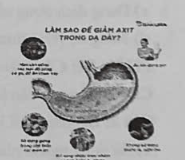
\includegraphics[width=0.35\textwidth]{images_crop/de504_da_day.png}
\end{center}
\loigiai{
- Ở trạng thái bình thường:
\[ \text{pH}_{\text{bình thường}} = -\log[\ce{H+}] = -\log(2 \cdot 10^{-4}) = 4 - \log 2 \approx 3{,}70. \]
- Khi dạ dày tiến hành tiêu hóa thức ăn:
\[ \text{pH}_{\text{tiêu hóa}} = -\log[\ce{H+}] = -\log(4 \cdot 10^{-2}) = 2 - \log 4 \approx 1{,}40. \]
\textbf{Đáp số:} Trạng thái bình thường $\text{pH} \approx 3{,}70$; khi tiêu hóa thức ăn $\text{pH} \approx 1{,}40$.}
\end{ex}

\bigskip
\noindent
{\color{hfRed}\textbf{\large BẢNG TỔNG HỢP ĐÁP ÁN ĐỀ SỐ 504}}

\smallskip
\noindent
\textbf{1. PHẦN I (Trắc nghiệm nhiều phương án):}
\begin{center}
\begin{tabular}{|c|c|c|c|c|c|c|c|c|c|c|c|}
\hline
\textbf{1. D} & \textbf{2. B} & \textbf{3. D} & \textbf{4. C} & \textbf{5. A} & \textbf{6. C} & \textbf{7. C} & \textbf{8. A} & \textbf{9. B} & \textbf{10. B} & \textbf{11. B} & \textbf{12. C} \\ \hline
\end{tabular}
\end{center}

\noindent
\textbf{2. PHẦN II (Trắc nghiệm đúng sai):}
\begin{itemize}
	\item \textbf{Câu 1:} a) Sai \quad|\quad b) Sai \quad|\quad c) Đúng \quad|\quad d) Đúng
	\item \textbf{Câu 2:} a) Đúng \quad|\quad b) Đúng \quad|\quad c) Sai \quad|\quad d) Sai
\end{itemize}

\noindent
\textbf{3. PHẦN III (Trả lời ngắn):}
\begin{center}
\begin{tabular}{|c|c|c|c|}
\hline
\textbf{Câu 1} & \textbf{Câu 2} & \textbf{Câu 3} & \textbf{Câu 4} \\ \hline
3 & 3 & 0,006 & 3 \\ \hline
\end{tabular}
\end{center}

\begin{center}
\textbf{--------- HẾT ---------}\\
\textit{(Học sinh không sử dụng tài liệu và bảng tuần hoàn hoá học)}
\end{center}

\end{document}
